\section{Contract Net Protocol}

\begin{frame}
	\frametitle{}
	
	\Huge
	
	\vspace{0.5cm}
	
	\begin{center}
		\textbf{Auctions}
	\end{center}
\end{frame}

\begin{frame}
	\frametitle{Auctions: Example}
	\framesubtitle{Environment}
	
	\vspace{0.27cm}
	
	\large
	
	Consider the following scenario in which there are:
	
	\begin{itemize}
		\item $ 2 $ teams of $ 3 $ robotic agents
		\vspace{0.1cm}
		\item $ 3 $ locations per team to be assigned (one position per agent)
			  \begin{itemize}
				  \vspace{0.05cm}
			  	  \item $ 2 $ are static in the field
				  \vspace{0.05cm}
			  	  \item $ 1 $ depends on the position of the ball
			  \end{itemize}
	\end{itemize}
	
	\vspace{-0.15cm}
	
	\begin{figure}[!h]
		\centering
		\begin{tikzpicture}[map/.style={draw=white,ultra thick,inner sep=0pt}]
			\node at (0,0) [map]
			{
				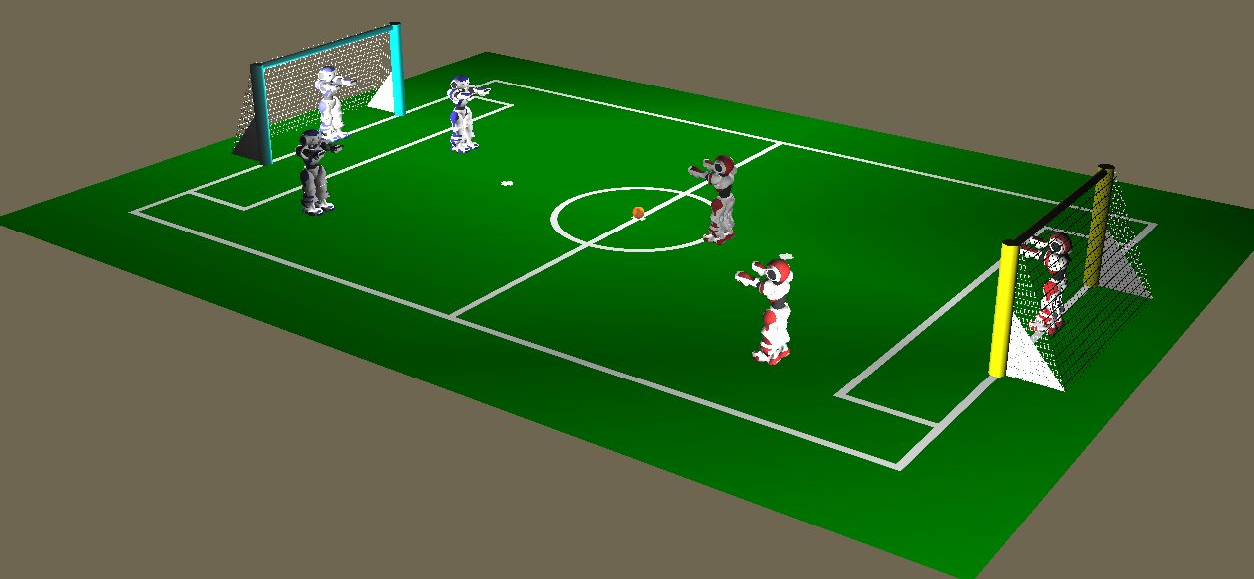
\includegraphics[width=0.73\linewidth]{Figures/SoccerField}
			};
		\end{tikzpicture}
	\end{figure}
\end{frame}

\begin{frame}
	\frametitle{Auctions: Example}
	
	\large
	
	\vspace{0.5cm}
	
	Let us assume the following initial configuration, where distances are calculated using the 
	Manhattan distance:
	
	\begin{table}[!h]
		\centering
		\setlength\tabcolsep{7pt}
		\def\arraystretch{1.3}
		\begin{tabular}{|c|c|c|c|c|c|c|c|c|c|c|}
			\hline
			&  & \textcolor{red}{$ a_{22} $} & & & \textcolor{red}{$ a_{23} $} &  & \textcolor{blue}{$ a_{12} $} &  &  &  \\ \hline
			
			&  &  & $ L_{12} $ &  &  & $ L_{22} $ &  & & \textcolor{red}{$ a_{21} $} & \\ \hline
			
			&  &  &  &  &  &  &  &  &  & \\ \hline
			
			$ L_{11} $ &  &  &  &  &  &  &  &  &  & $ L_{21} $ \\ \hline
			
			&  &  &  &  &  &  &  &  &  & \\ \hline
			
			&  &  &  & \textcolor{orange}{$ B $} &  &  &  &  & &  \\ \hline
			
			& \textcolor{blue}{$ a_{11} $} &  &  &  &  &  &  & \textcolor{blue}{$ a_{13} $} &  & \\ \hline
		\end{tabular}
	\end{table}
\end{frame}

\begin{frame}
	\frametitle{Auctions: Example - cont'd}
	
	\Large
	
	\begin{enumerate}
		\item Describe an utility function for the given problem
		\item Describe a simple auction protocol to let agents reach the goal of positioning
			  themselves in the best suitable position assuming:
			  
			  \begin{enumerate}
				  \item a static ball, no robot orientations
				  \item a static ball, robots oriented as follows (weight 50\%):
					  \begin{itemize}
						  \item $ a_{11} = 30\degree, a_{12} = 65\degree, a_{13} = 45\degree $
						  \item $ a_{21} = 60\degree, a_{22} = 35\degree, a_{23} = 80\degree $
					  \end{itemize}
				  \item ball moves \emph{West} until reaching the border, no robot orientations
			  \end{enumerate}
	\end{enumerate}
\end{frame}

\begin{frame}
	\frametitle{}
	
	\Large
	
	\vspace{0.7cm}
	
	\begin{center}
		\textbf{Case 1: static ball, no robot orientations}
	\end{center}
\end{frame}

\begin{frame}
	\frametitle{Auctions: Example Solution}
	\framesubtitle{Case 1 - Utility function}
	
	\large
	
	\vspace{0.5cm}
	
	\begin{equation*}
		u(A,L) = \alpha \Big [ 1 - \frac{Manhattan(A,L)}{MAX_{ROWS} \times MAX_{COLS}} \Big ] + \beta \Big [ 1 - \frac{| \theta_{target} |}{\pi} \Big ]
	\end{equation*}
	
	\vspace{0.3cm}
	
	where:
	
	\begin{itemize}
		\item $ \alpha = 1 $
		\item $ \beta = 0 $
	\end{itemize}
\end{frame}

\begin{frame}
	\frametitle{Auctions: Example Solution}
	\framesubtitle{Case 1 - Iteration 1}
	
	\vspace{0.3cm}
	
	\textbf{\underline{Auction run (step 1):}}
	
	\begin{itemize}
		\item<1-> $ a_{11} = \langle 0.948,0.909,0.948 \rangle $
		\item<1-> $ a_{12} = \langle 0.870,0.935,0.896 \rangle $ $ \;\;\;\;\;\;\;\;\; \leadsto
					\;\; \textcolor{blue}{\langle a_{11},B \rangle}, \textcolor{blue}{\langle
					a_{12},L_{12} \rangle}, \textcolor{blue}{\langle a_{13},L_{11} \rangle} $
		\item<1-> $ a_{13} = \langle 0.857,0.870,0.935 \rangle $
		\vspace{0.5cm}
		\item<2-> $ a_{21} = \langle 0.961,0.961,0.883 \rangle $
		\item<2-> $ a_{22} = \langle 0.857,0.935,0.909 \rangle $ $ \;\;\;\;\;\;\;\;\; \leadsto
					\;\; \textcolor{red}{\langle a_{23},B \rangle}, \textcolor{red}{\langle
					a_{21},L_{22} \rangle}, \textcolor{red}{\langle a_{22},L_{21} \rangle} $
		\item<2-> $ a_{23} = \langle 0.896,0.974,0.922 \rangle $
	\end{itemize}
\end{frame}

\begin{frame}
	\frametitle{Auctions: Example Solution}
	\framesubtitle{Case 1 - Iteration 1}
	
	\large
	
	\vspace{0.5cm}
	
	Environment state after iteration 1 is the following:
	
	\begin{table}[!h]
		\centering
		\setlength\tabcolsep{7pt}
		\def\arraystretch{1.3}
		\begin{tabular}{|c|c|c|c|c|c|c|c|c|c|c|}
			\hline
			&  & & & &  & \textcolor{blue}{$ a_{12} $} &  &  &  &  \\ \hline
			
			&  & \textcolor{red}{$ a_{22} $} & $ L_{12} $ &  & \textcolor{red}{$ a_{23} $} & $ L_{22} $ &  & \textcolor{red}{$ a_{21} $} & & \\ \hline
			
			&  &  &  &  &  &  &  &  &  & \\ \hline
			
			$ L_{11} $ &  &  &  &  &  &  &  &  &  & $ L_{21} $ \\ \hline
			
			&  &  &  &  &  &  &  &  &  & \\ \hline
			
			&  &  &  & \textcolor{orange}{$ B $} &  &  &  &  & &  \\ \hline
			
			& & \textcolor{blue}{$ a_{11} $} &  &  &  &  & \textcolor{blue}{$ a_{13} $} & &  & \\ \hline
		\end{tabular}
	\end{table}
\end{frame}

\begin{frame}
	\frametitle{Auctions: Example Solution}
	\framesubtitle{Case 1 - Iteration 2}
	
	\vspace{0.3cm}
	
	\textbf{\underline{Auction run (step 2):}}
	
	\begin{itemize}
		\item<1-> $ a_{11} = \langle 0.935,0.922,0.961 \rangle $
		\item<1-> $ a_{12} = \langle 0.883,0.948,0.909 \rangle $ $ \;\;\;\;\;\;\;\;\; \leadsto
					\;\; \textcolor{blue}{\langle a_{11},B \rangle}, \textcolor{blue}{\langle
					a_{12},L_{12} \rangle}, \textcolor{blue}{\langle a_{13},L_{11} \rangle} $
		\item<1-> $ a_{13} = \langle 0.870,0.883,0.948 \rangle $
		\vspace{0.5cm}
		\item<2-> $ a_{21} = \langle 0.948,0.974,0.896 \rangle $
		\item<2-> $ a_{22} = \langle 0.870,0.948,0.922 \rangle $ $ \;\;\;\;\;\;\;\;\; \leadsto
					\;\; \textcolor{red}{\langle a_{23},B \rangle}, \textcolor{red}{\langle
					a_{21},L_{22} \rangle}, \textcolor{red}{\langle a_{22},L_{21} \rangle} $
		\item<2-> $ a_{23} = \langle 0.909,0.987,0.935 \rangle $
	\end{itemize}
\end{frame}

\begin{frame}
	\frametitle{Auctions: Example Solution}
	\framesubtitle{Case 1 - Iteration 2}
	
	\large
	
	\vspace{0.5cm}
	
	Environment state after iteration 2 is the following:
	
	\begin{table}[!h]
		\centering
		\setlength\tabcolsep{7pt}
		\def\arraystretch{1.3}
		\begin{tabular}{|c|c|c|c|c|c|c|c|c|c|c|}
			\hline
			&  & & & & \textcolor{blue}{$ a_{12} $} & &  &  &  &  \\ \hline
			
			&  & & $ L_{12} $ &  & & $ L_{22} $ & \textcolor{red}{$ a_{21} $} & & & \\ \hline
			
			&  & \textcolor{red}{$ a_{22} $} &  &  & \textcolor{red}{$ a_{23} $} & &  &  &  & \\ \hline
			
			$ L_{11} $ &  &  &  &  &  &  &  &  &  & $ L_{21} $ \\ \hline
			
			&  &  &  &  &  &  &  &  &  & \\ \hline
			
			&  &  &  & \textcolor{orange}{$ B $} &  &  &  &  & &  \\ \hline
			
			& & & \textcolor{blue}{$ a_{11} $} &  &  & \textcolor{blue}{$ a_{13} $} & & &  & \\ \hline
		\end{tabular}
	\end{table}
\end{frame}

\begin{frame}
	\frametitle{Auctions: Example Solution}
	\framesubtitle{Execution trend}
	
	\Large
	
	Considering the first two iterations it is clear that:
	
	\vspace{0.1cm}
	
	\begin{enumerate}
		\item task assignment is:
			  \begin{itemize}
				  \vspace{0.1cm}
			  	  \item $ \textcolor{blue}{\langle a_{11},B \rangle}, \textcolor{blue}{\langle
						  a_{12},L_{12} \rangle}, \textcolor{blue}{\langle a_{13},L_{11}
						  \rangle} $
				  \vspace{0.1cm}
				  \item $ \textcolor{red}{\langle a_{23},B \rangle}, \textcolor{red}{\langle
				  		  a_{21},L_{22} \rangle}, \textcolor{red}{\langle a_{22},L_{21} \rangle}
				  		  $
			  \end{itemize}
		\vspace{0.1cm}
		\item agents will never change the task when executing it
	\end{enumerate}
\end{frame}

\begin{frame}
	\frametitle{}
	
	\Large
	
	\vspace{0.7cm}
	
	\begin{center}
		\textbf{Case 2: static ball, robots have an orientation}
	\end{center}
\end{frame}

\begin{frame}
	\frametitle{Auctions: Example Solution}
	\framesubtitle{Initial configuration}
	
	\large
	
	\vspace{0.5cm}
	
	Let us assume again the following initial configuration:
	
	\begin{table}[!h]
		\centering
		\setlength\tabcolsep{7pt}
		\def\arraystretch{1.3}
		\begin{tabular}{|c|c|c|c|c|c|c|c|c|c|c|}
			\hline
			&  & \textcolor{red}{$ a_{22} $} & & & \textcolor{red}{$ a_{23} $} &  & \textcolor{blue}{$ a_{12} $} &  &  &  \\ \hline
			
			&  &  & $ L_{12} $ &  &  & $ L_{22} $ &  & & \textcolor{red}{$ a_{21} $} & \\ \hline
			
			&  &  &  &  &  &  &  &  &  & \\ \hline
			
			$ L_{11} $ &  &  &  &  &  &  &  &  &  & $ L_{21} $ \\ \hline
			
			&  &  &  &  &  &  &  &  &  & \\ \hline
			
			&  &  &  & \textcolor{orange}{$ B $} &  &  &  &  & &  \\ \hline
			
			& \textcolor{blue}{$ a_{11} $} &  &  &  &  &  & & \textcolor{blue}{$ a_{13} $} &  & \\ \hline
		\end{tabular}
	\end{table}
\end{frame}

\begin{frame}
	\frametitle{Auctions: Example Solution}
	\framesubtitle{Case 2 - Utility function}
	
	\large
	
	\vspace{0.5cm}
	
	\begin{equation*}
		u(A,L) = \alpha \Big [ 1 - \frac{Manhattan(A,L)}{MAX_{ROWS} \times MAX_{COLS}} \Big ] + \beta \Big [ 1 - \frac{| \theta_{target} |}{\pi} \Big ]
	\end{equation*}
	
	\vspace{0.3cm}
	
	where:
	
	\begin{itemize}
		\item $ \alpha = 0.5 $
		\item $ \beta = 0.5 $
	\end{itemize}
\end{frame}

\begin{frame}
	\frametitle{Auctions: Example Solution}
	\framesubtitle{Case 2 - Iteration 1}
	
	\vspace{0.3cm}
	
	\textbf{\underline{Auction run (step 1):}}
	
	\begin{itemize}
		\item<1-> $ a_{11} = \langle 0.941,0.813,0.693 \rangle $
		\item<1-> $ a_{12} = \langle 0.799,0.856,0.712 \rangle $ $ \;\;\;\;\;\;\;\;\;
					\leadsto \;\; \textcolor{blue}{\langle a_{13},B \rangle}, \textcolor{blue}
					{\langle a_{12},L_{12} \rangle}, \textcolor{blue}{\langle a_{11},L_{11}
					\rangle} $
		\item<1-> $ a_{13} = \langle 0.859,0.935,0.898 \rangle $
		\vspace{0.5cm}
		\item<2-> $ a_{21} = \langle 0.578,0.897,0.750 \rangle $
		\item<2-> $ a_{22} = \langle 0.532,0.579,0.468 \rangle $ $ \;\;\;\;\;\;\;\;\; \leadsto
					\;\; \textcolor{red}{\langle a_{21},B \rangle}, \textcolor{red}{\langle
					a_{23},L_{22} \rangle}, \textcolor{red}{\langle a_{22},L_{21} \rangle} $
		\item<2-> $ a_{23} = \langle 0.504,0.584,0.711 \rangle $
	\end{itemize}
\end{frame}

\begin{frame}
	\frametitle{Auctions: Example Solution}
	\framesubtitle{Case 2 - Iteration 1}
	
	\large
	
	\vspace{0.5cm}
	
	Environment state after iteration 1 is the following:
	
	\begin{table}[!h]
		\centering
		\setlength\tabcolsep{7pt}
		\def\arraystretch{1.3}
		\begin{tabular}{|c|c|c|c|c|c|c|c|c|c|c|}
			\hline
			&  & & & & & \textcolor{blue}{$ a_{12} $} & &  &  &  \\ \hline
			
			&  & \textcolor{red}{$ a_{22} $} & $ L_{12} $ &  & \textcolor{red}{$ a_{23} $} & $ L_{22} $ &  & \textcolor{red}{$ a_{21} $} & & \\ \hline
			
			&  &  &  &  &  &  &  &  &  & \\ \hline
			
			$ L_{11} $ &  &  &  &  &  &  &  &  &  & $ L_{21} $ \\ \hline
			
			&  &  &  &  &  &  &  &  &  & \\ \hline
			
			& \textcolor{blue}{$ a_{11} $} &  &  & \textcolor{orange}{$ B $} &  &  &  &  & &  \\ \hline
			
			& &  &  &  &  &  & \textcolor{blue}{$ a_{13} $} & &  & \\ \hline
		\end{tabular}
	\end{table}
\end{frame}

\begin{frame}
	\frametitle{Auctions: Example Solution}
	\framesubtitle{Case 2 - Iteration 2}
	
	\Large
	
	\begin{center}
		\textbf{Do the same math over and over...} \\
		
		\vspace{0.5cm}
		
		\textbf{Verify at home whether tasks switch among agents!}
	\end{center}
\end{frame}

\begin{frame}
	\frametitle{}
	
	\Large
	
	\vspace{0.7cm}
	
	\begin{center}
		\textbf{Case 3: moving ball, no robot orientations}
	\end{center}
\end{frame}

\begin{frame}
	\frametitle{}
	
	\vspace{0.5cm}
	
	\begin{figure}[!h]
		\centering
		\begin{tikzpicture}[map/.style={draw=white,ultra thick,inner sep=0pt}]
			\node at (0,0) [map]
			{
				
\includegraphics[width=0.8\linewidth]{Figures/Homework}
			};
		\end{tikzpicture}
	\end{figure}
	
	\Huge
	
	\vspace{-0.55cm}
	
	\begin{center}
		...entirely at home!
	\end{center}
\end{frame}